\subsection{Driven Simple Harmonic Oscillator with Damping}

\subsubsection{Brief Derivation}
Let us define a Simple Harmonic Oscillator (SHO) of mass \(m\) and is attached to a spring with spring constant \(k\).
The SHO is subject to a damping force with damping coefficient \(\gamma\) and an additional driving force \(f(t)\).

\vspace{5mm}

Define \(\omega_0 = \sqrt{\frac{k}{m}}\) as the natural frequency of the SHO and the damping force as \(F_d = -2 m \gamma v\), where \(v\) is the velocity of the SHO.

\noindent
Using Newton's Second Law,
\begin{align}
    \Sigma F = ma &= -m \omega_0^2 x - 2 m \gamma v + f(t) \\
    m \frac{d^2 x}{dt^2} &= -m \omega_0^2 x - 2 m \gamma \frac{dx}{dt} + f(t)
\end{align}

\noindent
Dividing by \(m\) and rearranging terms, we get the following differential equation for a driven SHO with damping:

\begin{equation} \label{eq:driven_sho_equation}
    \frac{d^2 x}{dt^2} + 2 \gamma \frac{dx}{dt} + \omega_0^2 x(t) = \frac{f(t)}{m}
\end{equation}

\subsubsection{Application of the Fourier Transform}
\noindent
Let us take the Fourier Transform of \cref{eq:driven_sho_equation} with respect to \(t\). Thus, let \(X(\omega)\) be the Fourier Transform of \(x(t)\) and \(F(\omega)\) be the Fourier Transform of \(f(t)\).

\begin{equation}
    \mathcal{F} \left\{ \frac{d^2 x}{dt^2} + 2 \gamma \frac{dx}{dt} + \omega_0^2 x(t) \right\} = \mathcal{F} \left\{ \frac{f(t)}{m} \right\}
\end{equation}

\noindent
Using \cref{fourier_linearity},
\begin{equation} 
    \mathcal{F} \left\{ \frac{d^2 x}{dt^2} \right\} + \mathcal{F} \left\{ 2 \gamma \frac{dx}{dt} \right\} + \mathcal{F} \left\{ \omega_0^2 x(t) \right\} = \mathcal{F} \left\{ \frac{f(t)}{m} \right\}
\end{equation}

\noindent
Using \cref{fourier_scaling},
\begin{equation} 
    \mathcal{F} \left\{ \frac{d^2 x}{dt^2} \right\} + 2 \gamma \mathcal{F} \left\{ \frac{dx}{dt} \right\} + \omega_0^2 \mathcal{F} \left\{ x(t) \right\} = \frac{\mathcal{F} \left\{ f(t) \right\}}{m} 
\end{equation}

\noindent
Using \cref{fourier_derivative},
\begin{align}
    \mathcal{F} \left\{ \frac{dx}{dt} \right\} &= i \omega \mathcal{F} \left\{ x(t) \right\} \\
    &= i \omega X(\omega) \\
    \mathcal{F} \left\{ \frac{d^2 x}{d t^2} \right\} & = i \omega \mathcal{F} \left\{ \frac{dx}{dt} \right\} \\
    & = -\omega^2 X(\omega)
\end{align}

\noindent
Therefore,
\begin{align}
    -\omega^2 X(\omega) + 2 \gamma i \omega X(\omega) + \omega_0^2 X(\omega) &= \frac{F(\omega)}{m} \\
    X(\omega) \left( \omega_0^2 - \omega^2 + 2 \gamma i \omega \right) &= \frac{F(\omega)}{m}
\end{align}

\noindent
Thus,
\begin{equation} \label{eq:driven_sho_fourier}
    X(\omega) = \frac{F(\omega)}{m \left( \omega_0^2 - \omega^2 + 2 \gamma i \omega \right)}
\end{equation}

% TODO: Maybe make a section on summarizing the solving procedure and explaining exactly how the Fourier Transform helps us solve the ODE/PDE.
By applying the Fourier Transform to the driven SHO equation, we have reduced the problem from solving a second order ODE (\cref{eq:driven_sho_equation}) to solving a simple algebraic equation (\cref{eq:driven_sho_fourier}). This is a significant reduction in complexity.

Once we have solved for \(X(\omega)\), we can take the inverse Fourier Transform of \cref{eq:driven_sho_fourier} to obtain \(x(t)\).

\begin{align} \label{eq:driven_sho_inverse_fourier}
    x(t) &= \frac{1}{2 \pi} \int_{-\infty}^{\infty} X(\omega) e^{i \omega t} d\omega \\
    &= \frac{1}{2 \pi} \int_{-\infty}^{\infty} \frac{F(\omega)}{m \left( \omega_0^2 - \omega^2 + 2 \gamma i \omega \right)} e^{i \omega t} d\omega
\end{align}

\subsubsection{Boundary Conditions} % TODO: Add boundary conditions to the driven SHO equation.

\subsubsection{Numerical Solution to Driven SHO with Damping Equation}
\cref{eq:driven_sho_inverse_fourier} can be easily solved numerically using the Fast Fourier Transform (FFT) and the Inverse Fast Fourier Transfrom (IFFT) algorithms. The FFT and IFFT algorithms are optimized algorithms for computing the Discrete Fourier Transform (DFT) and the Inverse Discrete Fourier Transform (IDFT) of a sequence.

\begin{figure}[H]
    \centering
    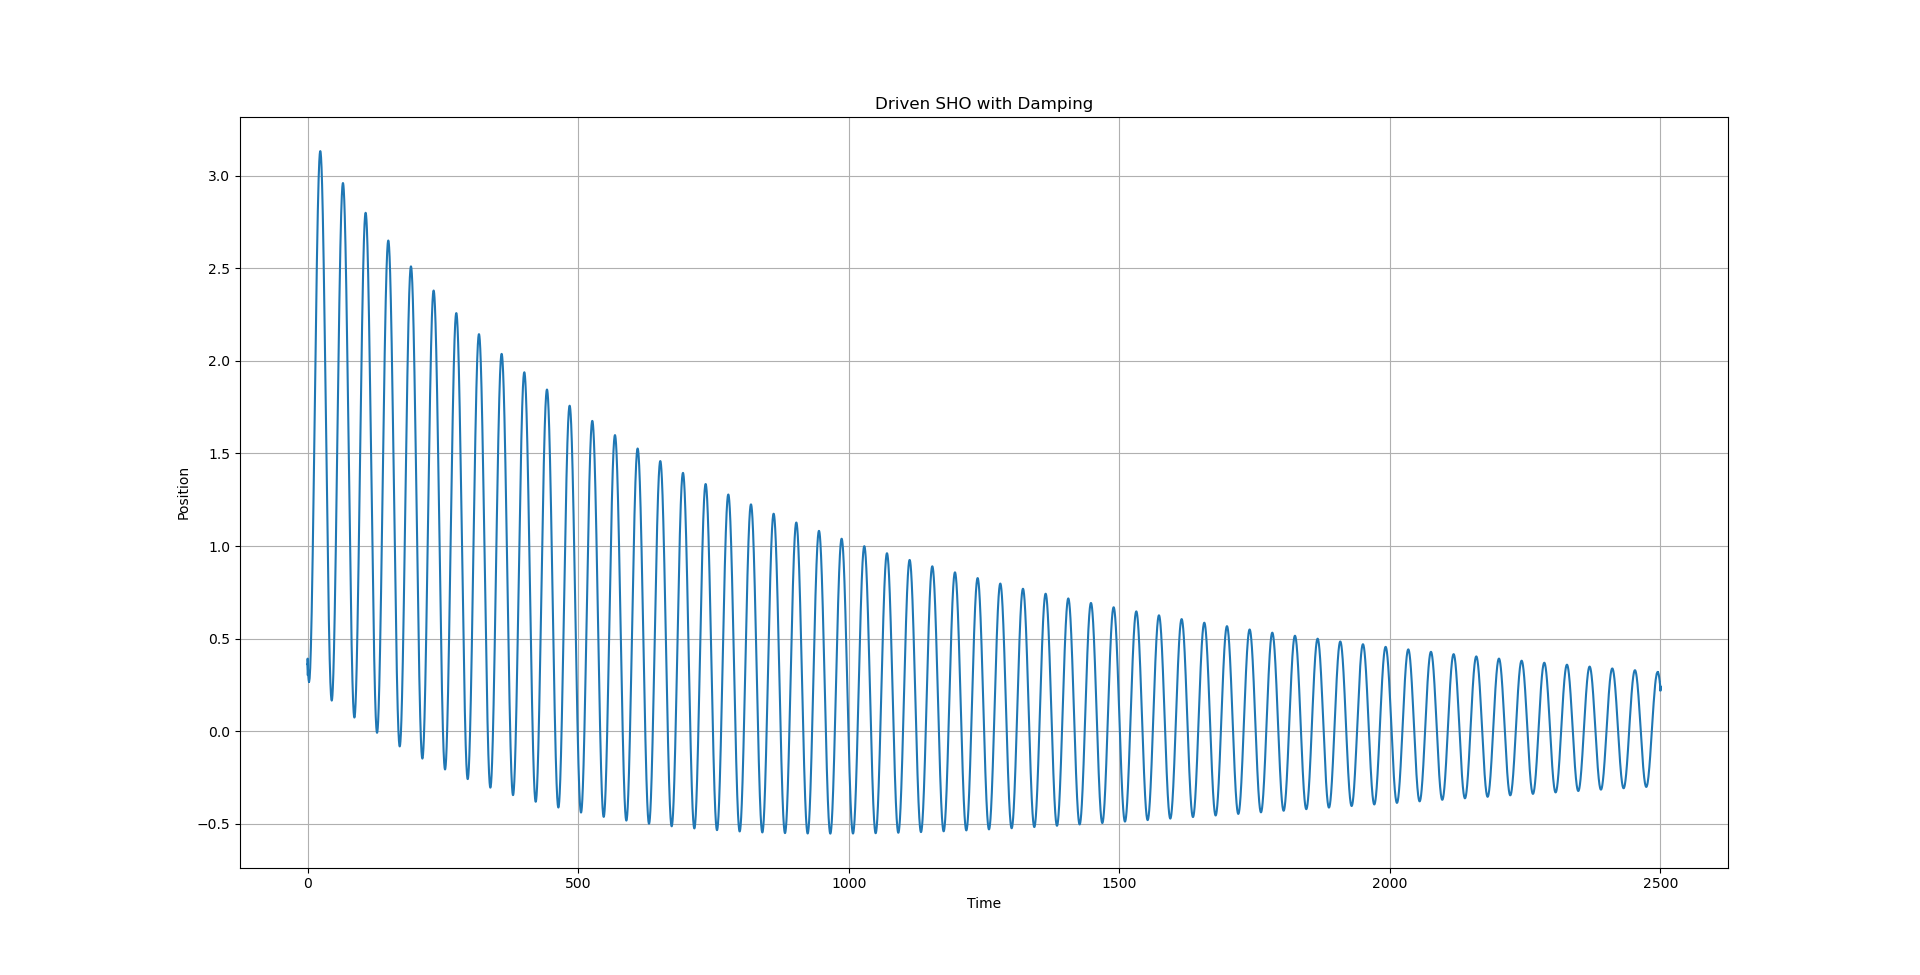
\includegraphics[width=110mm,height=\textheight,keepaspectratio]{images/driven_sho_equation_numerical.png}
    \caption{Defining the SHO parameters such that \(m=1\), \(\omega_0=0.15\), \(\gamma=0.005\), and \(f(t)=2 \sin (\omega_0 t)\), above is the solution to the driven SHO equation with damping using the FFT and IFFT algorithms in Python.}
    \label{fig:driven_sho_equation_numerical}
\end{figure}


% \subsubsection{Analytical Solution to Wave Equation} 
% This is a maybe section. Possibly replace this section with a section on the applicability of the Fourier Transform to reduce PDEs to ODEs...?